\section*{Appendix A: Detailed Information on Open-Ended Responses and Discursive Sophistication Components}
\renewcommand\thefigure{A.\arabic{figure}}
\renewcommand\thetable{A.\arabic{table}}
\setcounter{figure}{0}
\setcounter{table}{0}

\begin{figure*}[h]
    \centering
    \begin{subfigure}[t]{0.49\textwidth}
        \centering
        \includegraphics{/data/Dropbox/Uni/Projects/2016/knowledge/fig/anes2012_wc.pdf}
        \caption{2012 ANES}
    \end{subfigure}%
	\begin{subfigure}[t]{0.49\textwidth}
        \centering
        \includegraphics{/data/Dropbox/Uni/Projects/2016/knowledge/fig/anes2016_wc.pdf}
        \caption{2016 ANES}
    \end{subfigure}%
    
    \begin{subfigure}[t]{0.49\textwidth}
        \centering
        \includegraphics{/data/Dropbox/Uni/Projects/2016/knowledge/fig/yg_wc.pdf}
        \caption{2015 YouGov}
    \end{subfigure}
    \begin{subfigure}[t]{0.49\textwidth}
         \centering
         \includegraphics{/data/Dropbox/Uni/Projects/2016/knowledge/fig/swiss_wc.pdf}
         \caption{Swiss Survey}
    \end{subfigure}
    \caption{Histograms of total word count in the collection of open-ended responses for each individual. The dashed red lines indicate the average response lengths in each survey.}\label{fig:wc}
\end{figure*}

\begin{figure}[h]\centering
\includegraphics[width=\textwidth]{/data/Dropbox/Uni/Projects/2016/knowledge/fig/anes_stm_prop.pdf}
\caption{Estimated topic proportions in the 2012 and 2016 ANES based on the structural topic model. See Appendix B for details on the model specification.}\label{fig:anes_stm_prop}
\end{figure}

\begin{figure}[h]\centering
\includegraphics[width=.5\textwidth]{/data/Dropbox/Uni/Projects/2016/knowledge/fig/yg_stm_prop.pdf}
\caption{Estimated topic proportions in the 2015 YouGov survey based on the structural topic model. See Appendix B for details on the model specification.}\label{fig:yg_stm_prop}
\end{figure}

\begin{figure}[h]\centering
\includegraphics[width=\textwidth]{/data/Dropbox/Uni/Projects/2016/knowledge/fig/swiss_stm_prop.pdf}
\caption{Estimated topic proportions in the Swiss survey based on the structural topic model. See Appendix B for details on the model specification.}\label{fig:swiss_stm_prop}
\end{figure}

\begin{figure*}[h]
    \centering
    \begin{subfigure}[h]{0.5\textwidth}
        \centering
        \includegraphics{/data/Dropbox/Uni/Projects/2016/knowledge/fig/anes2012_corplot_components.pdf}
        \caption{2012 ANES}
    \end{subfigure}%
    \begin{subfigure}[h]{0.5\textwidth}
         \centering
         \includegraphics{/data/Dropbox/Uni/Projects/2016/knowledge/fig/anes2016_corplot_components.pdf}
         \caption{2016 ANES}
    \end{subfigure}%
    
    \begin{subfigure}[h]{0.49\textwidth}
        \centering
        \includegraphics{/data/Dropbox/Uni/Projects/2016/knowledge/fig/yg_corplot_components.pdf}
        \caption{2015 YouGov}
    \end{subfigure}
    \begin{subfigure}[h]{0.49\textwidth}
         \centering
         \includegraphics{/data/Dropbox/Uni/Projects/2016/knowledge/fig/swiss_corplot_components.pdf}
         \caption{Swiss Survey}
    \end{subfigure}
    \caption{Correlation matrix of individual components of discursive sophistication. The plots on the diagonal display univariate densities for each component. The panels in the lower triangular display the scatter plot of two measures as well as a linear fit. The upper triangular displays the correlation coefficient.}\label{fig:components}
\end{figure*}



\clearpage
\section*{Appendix B: Pre-Processing and Topic Model Specification}
\renewcommand\thefigure{B.\arabic{figure}}
\renewcommand\thetable{B.\arabic{table}}
\setcounter{figure}{0}
\setcounter{table}{0}

Two components of discursive sophistication (\textit{considerations} and \textit{word choice}) rely on quantities extracted from structural topic models \citep{roberts2014structural}. As with any other text-as-data approach, a necessary first step before estimating the topic model is to pre-process the raw text and convert it into a document term matrix \citep[DTM, see for example][]{manning2008introduction}. Common pre-processing procedures include stemming and lowercasing, as well as the removal of numbers, punctuation, stopwords, and infrequent terms. However, topic models and other unsupervised learning techniques can be sensitive to these pre-processing choices \citep[c.f.,][]{denny2018text}. To address this issue, \citet{denny2018text} recommend that researchers compare DTMs under all possible pre-processing regimes. The authors propose \textit{preText scores} as a measure to quantify the extent to which varying pre-processing regimes may yield unusual results compared to a baseline without any pre-processing.

\begin{figure}[h]
\centering\includegraphics{/data/Dropbox/Uni/Projects/2016/knowledge/fig/pretext.pdf}
    \caption{PreText analysis of pre-processing decisions of open-ended responses across all datasets. Regression coefficients display the effects of each of the six pre-processing choices on the resulting preText score.}\label{fig:pretext}
\end{figure}

Following the procedure outlined in \citet{denny2018text}, Figure~\ref{fig:pretext} displays the results of a linear model regressing preText scores resulting from all possible pre-processing regimes on each individual step for a random subset of 500 open-ended responses in each of the studies included in the analyses. Significant coefficients indicate that the topic model results my be sensitive to the respective pre-processing step. As such, removing stopwords and punctuation, as well as removing infrequent terms (at least in the 2016 ANES) might be problematic. \citet{denny2018text}, however, emphasize that the most important consideration in choosing pre-processing steps are theoretical. Given that the purpose of the topic model is to extract considerations related to political preferences, there are strong theoretical reasons to remove stopwords and punctuation from open-ended responses as they do not contain any relevant content. Furthermore, I apply lowercasing and stemming of terms to reduce resulting document term matrix to a computationally more manageable size and since these pre-processing steps should not be influential according to the preText analysis.

It is less obvious from a theoretical perspective whether to remove infrequent terms from open-ended responses, although it is preferred in order to make the estimation of the discursive sophistication components computationally efficient. Since the preText analysis for the 2016 ANES suggests that this pre-processing step might be influential, I compare discursive sophistication for both alternative regimes below \citep[c.f.,][]{denny2018text}. Before turning to this sensitivity check, however, I consider another crucial modeling choice when working with topic models: determining the total number of topics $k$ to be estimated. For all analyses reported below, the number of topics was selected using the algorithm proposed by \citet{lee2014low} and implemented in the \texttt{stm} package in \textbf{R} \citep{roberts2014stm}.\footnote{I used measures for age, gender, education, party identification, as well as an interaction between education and party identification as covariates for topic prevalence. This variable selection---with the exception of including gender---is equivalent to the procedure model specification described in \citet{roberts2014structural}.} 

\begin{figure}[h]\centering
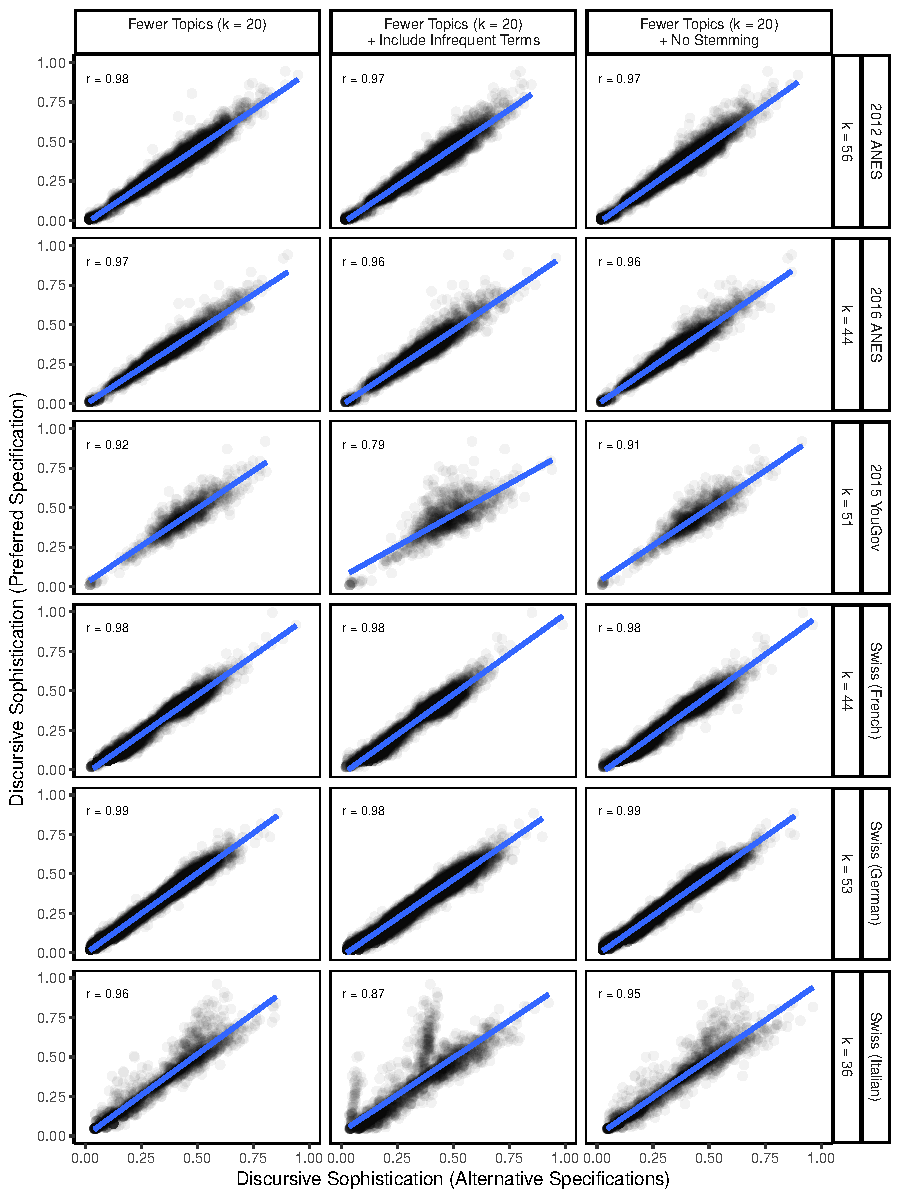
\includegraphics{/data/Dropbox/Uni/Projects/2016/knowledge/fig/pretext_robustness.pdf}
\caption{Robustness of discursive sophistication measure for different pre-processing choices and topic model specifications.}\label{fig:pretext_robustness}
\end{figure}

Figure~\ref{fig:pretext_robustness} examines whether the proposed measure of discursive sophistication is sensitive to the removal of infrequent terms as well as the chosen number of topics $k$. The y-axis depicts the preferred pre-processing regime including all steps discussed above while the x-axis plots results for alternative specifications. The panels on the left compare the preferred specification to discursive sophistication based on a reduced number of topics ($k=20$). The middle panels additionally include infrequent terms instead of removing them.\footnote{Calculating discursive sophistication with large numbers of topics while including infrequent terms is computationally prohibitive.} The panels on the right omit do not perform stemming as part of the pre-processing step. Across all panels, discursive sophistication scores are highly correlated and therefore insensitive to pre-processing choices and varying numbers of topics.

In summary, open-ended responses in the analyses reported below are pre-processed by stemming and lowercasing, as well as the removing numbers, punctuation, stopwords, and infrequent terms (i.e., terms that appear in fewer than 10 responses).\footnote{Prior to applying these pre-processing steps, open-ended responses in the 2012 \& 2016 ANES as well as the 2015 YouGov survey are cleaned by correcting spelling errors using an implementation of the Aspell spell-checking algorithm (\url{www.aspell.net}).} While the results discussed in the manuscript are based on this preferred specification, the substantive results are robust for alternative pre-processing regimes or varying numbers of topics.


%\clearpage
%\section*{Appendix C: Tables of Model Estimates}
%\renewcommand\thefigure{C.\arabic{figure}}
%\renewcommand\thetable{C.\arabic{table}}
%\setcounter{figure}{0}
%\setcounter{table}{0}
%
%
% Table created by stargazer v.5.2 by Marek Hlavac, Harvard University. E-mail: hlavac at fas.harvard.edu
% Date and time: Mon, Apr 03, 2017 - 04:16:03 PM
% Requires LaTeX packages: dcolumn 
\begin{table}[ht] \centering 
  \caption{Effects of sophistication -- OLS models predicting internal efficacy 
          based on different sophistication 
          measures. Positive coefficients indicate higher self-reported internal efficacy. 
          Standard errors in parentheses. Estimates are used for Figure~\ref{fig:knoweff} 
          in the main text.} 
  \label{tab:inteff} 
\scriptsize 
\begin{tabular}{@{\extracolsep{-5pt}}lD{.}{.}{-3} D{.}{.}{-3} D{.}{.}{-3} D{.}{.}{-3} D{.}{.}{-3} D{.}{.}{-3} } 
\\[-1.8ex]\hline 
\hline \\[-1.8ex] 
 & \multicolumn{6}{c}{\textit{Dependent variable:}} \\ 
\cline{2-7} 
\\[-1.8ex] & \multicolumn{6}{c}{Iternal Efficacy} \\ 
\\[-1.8ex] & \multicolumn{1}{c}{(1)} & \multicolumn{1}{c}{(2)} & \multicolumn{1}{c}{(3)} & \multicolumn{1}{c}{(4)} & \multicolumn{1}{c}{(5)} & \multicolumn{1}{c}{(6)}\\ 
\hline \\[-1.8ex] 
 Text-based & 0.554^{***} &  &  &  &  &  \\ 
  & (0.035) &  &  &  &  &  \\ 
  Factual &  & 0.237^{***} &  &  &  &  \\ 
  &  & (0.015) &  &  &  &  \\ 
  Office &  &  & 0.248^{***} &  &  &  \\ 
  &  &  & (0.011) &  &  &  \\ 
  Majorities &  &  &  & 0.140^{***} &  &  \\ 
  &  &  &  & (0.008) &  &  \\ 
  Eval. (Pre) &  &  &  &  & 0.361^{***} &  \\ 
  &  &  &  &  & (0.019) &  \\ 
  Eval. (Post) &  &  &  &  &  & 0.285^{***} \\ 
  &  &  &  &  &  & (0.020) \\ 
  Sex (Female) & -0.062^{***} & -0.050^{***} & -0.052^{***} & -0.053^{***} & -0.038^{***} & -0.040^{***} \\ 
  & (0.006) & (0.006) & (0.006) & (0.006) & (0.010) & (0.010) \\ 
  Education (College) & 0.056^{***} & 0.055^{***} & 0.038^{***} & 0.063^{***} & 0.035^{**} & 0.044^{***} \\ 
  & (0.006) & (0.006) & (0.007) & (0.006) & (0.011) & (0.012) \\ 
  log(Age) & 0.019^{*} & 0.008 & 0.009 & 0.010 & -0.016 & -0.005 \\ 
  & (0.008) & (0.008) & (0.008) & (0.008) & (0.012) & (0.013) \\ 
  Race (Black) & 0.041^{***} & 0.058^{***} & 0.048^{***} & 0.042^{***} & 0.050^{***} & 0.059^{***} \\ 
  & (0.008) & (0.008) & (0.008) & (0.008) & (0.011) & (0.011) \\ 
  Church Attendance & 0.005 & 0.008 & 0.013 & 0.005 & -0.003 & -0.009 \\ 
  & (0.008) & (0.008) & (0.008) & (0.009) & (0.014) & (0.015) \\ 
  Survey Mode (Online) & 0.047^{***} & 0.009 & -0.009 & 0.001 &  &  \\ 
  & (0.006) & (0.006) & (0.007) & (0.007) &  &  \\ 
  Constant & 0.179^{***} & 0.368^{***} & 0.442^{***} & 0.444^{***} & 0.377^{***} & 0.400^{***} \\ 
  & (0.033) & (0.030) & (0.030) & (0.031) & (0.044) & (0.047) \\ 
 \hline \\[-1.8ex] 
Observations & \multicolumn{1}{c}{5,135} & \multicolumn{1}{c}{5,135} & \multicolumn{1}{c}{4,816} & \multicolumn{1}{c}{4,816} & \multicolumn{1}{c}{1,743} & \multicolumn{1}{c}{1,647} \\ 
R$^{2}$ & \multicolumn{1}{c}{0.114} & \multicolumn{1}{c}{0.116} & \multicolumn{1}{c}{0.160} & \multicolumn{1}{c}{0.128} & \multicolumn{1}{c}{0.228} & \multicolumn{1}{c}{0.170} \\ 
\hline 
\hline \\[-1.8ex] 
\textit{Note:}  & \multicolumn{6}{r}{$^{*}$p$<$0.05; $^{**}$p$<$0.01; $^{***}$p$<$0.001} \\ 
\end{tabular} 
\end{table} 

%
% Table created by stargazer v.5.2 by Marek Hlavac, Harvard University. E-mail: hlavac at fas.harvard.edu
% Date and time: Fri, Mar 31, 2017 - 11:40:42 PM
% Requires LaTeX packages: dcolumn 
\begin{table}[ht] \centering 
  \caption{Effects on External Efficacy} 
  \label{tab:exteff} 
\scriptsize 
\begin{tabular}{@{\extracolsep{-5pt}}lD{.}{.}{-3} D{.}{.}{-3} D{.}{.}{-3} D{.}{.}{-3} D{.}{.}{-3} D{.}{.}{-3} } 
\\[-1.8ex]\hline 
\hline \\[-1.8ex] 
 & \multicolumn{6}{c}{\textit{Dependent variable:}} \\ 
\cline{2-7} 
\\[-1.8ex] & \multicolumn{6}{c}{External Efficacy} \\ 
\hline \\[-1.8ex] 
 Text-based & 0.130^{**} &  &  &  &  &  \\ 
  & (0.040) &  &  &  &  &  \\ 
  Factual &  & 0.059^{***} &  &  &  &  \\ 
  &  & (0.017) &  &  &  &  \\ 
  Office &  &  & 0.089^{***} &  &  &  \\ 
  &  &  & (0.013) &  &  &  \\ 
  Majorities &  &  &  & 0.045^{***} &  &  \\ 
  &  &  &  & (0.009) &  &  \\ 
  Eval. (Pre) &  &  &  &  & 0.139^{***} &  \\ 
  &  &  &  &  & (0.025) &  \\ 
  Eval. (Post) &  &  &  &  &  & 0.147^{***} \\ 
  &  &  &  &  &  & (0.026) \\ 
  Sex (Female) & 0.015^{*} & 0.018^{**} & 0.017^{*} & 0.016^{*} & 0.026^{*} & 0.025 \\ 
  & (0.007) & (0.007) & (0.007) & (0.007) & (0.013) & (0.013) \\ 
  Education (College) & 0.045^{***} & 0.045^{***} & 0.035^{***} & 0.045^{***} & 0.064^{***} & 0.057^{***} \\ 
  & (0.007) & (0.007) & (0.008) & (0.007) & (0.015) & (0.015) \\ 
  log(Age) & -0.006 & -0.009 & -0.013 & -0.012 & -0.052^{**} & -0.050^{**} \\ 
  & (0.009) & (0.009) & (0.009) & (0.009) & (0.016) & (0.017) \\ 
  Race (Black) & 0.073^{***} & 0.077^{***} & 0.076^{***} & 0.074^{***} & 0.052^{***} & 0.056^{***} \\ 
  & (0.009) & (0.009) & (0.009) & (0.009) & (0.014) & (0.015) \\ 
  Church Attendance & 0.050^{***} & 0.051^{***} & 0.055^{***} & 0.052^{***} & 0.049^{**} & 0.046^{*} \\ 
  & (0.009) & (0.009) & (0.010) & (0.010) & (0.019) & (0.019) \\ 
  Survey Mode (Online) & -0.034^{***} & -0.043^{***} & -0.056^{***} & -0.052^{***} &  &  \\ 
  & (0.007) & (0.007) & (0.008) & (0.008) &  &  \\ 
  Constant & 0.358^{***} & 0.403^{***} & 0.440^{***} & 0.439^{***} & 0.464^{***} & 0.467^{***} \\ 
  & (0.038) & (0.035) & (0.036) & (0.036) & (0.059) & (0.061) \\ 
 \hline \\[-1.8ex] 
Observations & \multicolumn{1}{c}{5,123} & \multicolumn{1}{c}{5,123} & \multicolumn{1}{c}{4,803} & \multicolumn{1}{c}{4,803} & \multicolumn{1}{c}{1,732} & \multicolumn{1}{c}{1,634} \\ 
R$^{2}$ & \multicolumn{1}{c}{0.040} & \multicolumn{1}{c}{0.041} & \multicolumn{1}{c}{0.049} & \multicolumn{1}{c}{0.045} & \multicolumn{1}{c}{0.054} & \multicolumn{1}{c}{0.053} \\ 
\hline 
\hline \\[-1.8ex] 
\textit{Note:}  & \multicolumn{6}{r}{$^{*}$p$<$0.05; $^{**}$p$<$0.01; $^{***}$p$<$0.001} \\ 
\end{tabular} 
\end{table} 

%
% Table created by stargazer v.5.2 by Marek Hlavac, Harvard University. E-mail: hlavac at fas.harvard.edu
% Date and time: Thu, Jun 22, 2017 - 04:21:46 PM
% Requires LaTeX packages: dcolumn 
\begin{table}[ht] \centering 
  \caption{Effects of sophistication -- OLS models predicting non-conventional 
          particpation (protest, signing 
          petitions, etc.) based on different sophistication 
          measures. Positive coefficients indicate higher levels of participation. 
          Standard errors in parentheses. Estimates are used for Figure~\ref{fig:knoweff} 
          in the main text.} 
  \label{tab:nonconv} 
\scriptsize 
\begin{tabular}{@{\extracolsep{-5pt}}lD{.}{.}{-3} D{.}{.}{-3} D{.}{.}{-3} D{.}{.}{-3} D{.}{.}{-3} D{.}{.}{-3} } 
\\[-1.8ex]\hline 
\hline \\[-1.8ex] 
 & \multicolumn{6}{c}{\textit{Dependent variable:}} \\ 
\cline{2-7} 
\\[-1.8ex] & \multicolumn{6}{c}{Non-conventional Participation} \\ 
\hline \\[-1.8ex] 
 Text-based & 1.124^{***} &  &  &  &  &  \\ 
  & (0.085) &  &  &  &  &  \\ 
  Factual &  & 0.193^{***} &  &  &  &  \\ 
  &  & (0.037) &  &  &  &  \\ 
  Office &  &  & 0.322^{***} &  &  &  \\ 
  &  &  & (0.028) &  &  &  \\ 
  Majorities &  &  &  & 0.151^{***} &  &  \\ 
  &  &  &  & (0.020) &  &  \\ 
  Eval. (Pre) &  &  &  &  & 0.453^{***} &  \\ 
  &  &  &  &  & (0.050) &  \\ 
  Eval. (Post) &  &  &  &  &  & 0.451^{***} \\ 
  &  &  &  &  &  & (0.050) \\ 
  Sex (Female) & 0.010 & 0.017 & 0.025 & 0.021 & 0.033 & 0.036 \\ 
  & (0.014) & (0.015) & (0.014) & (0.015) & (0.025) & (0.025) \\ 
  Education (College) & 0.082^{***} & 0.110^{***} & 0.082^{***} & 0.111^{***} & 0.103^{***} & 0.096^{**} \\ 
  & (0.017) & (0.017) & (0.017) & (0.016) & (0.030) & (0.030) \\ 
  Income & 0.063^{*} & 0.082^{**} & 0.048 & 0.087^{***} & 0.036 & 0.040 \\ 
  & (0.026) & (0.027) & (0.026) & (0.026) & (0.046) & (0.046) \\ 
  log(Age) & 0.036 & 0.038 & 0.026 & 0.031 & -0.057 & -0.054 \\ 
  & (0.019) & (0.020) & (0.019) & (0.020) & (0.031) & (0.031) \\ 
  Race (Black) & 0.040^{*} & 0.048^{*} & 0.042^{*} & 0.037 & -0.020 & -0.012 \\ 
  & (0.019) & (0.019) & (0.019) & (0.019) & (0.028) & (0.028) \\ 
  Church Attendance & 0.025 & 0.032 & 0.038 & 0.028 & 0.046 & 0.041 \\ 
  & (0.020) & (0.021) & (0.020) & (0.020) & (0.036) & (0.036) \\ 
  Survey Mode (Online) & 0.105^{***} & 0.055^{***} & 0.024 & 0.041^{*} &  &  \\ 
  & (0.016) & (0.016) & (0.016) & (0.016) &  &  \\ 
  Constant & -0.415^{***} & 0.008 & 0.108 & 0.092 & 0.270^{*} & 0.284^{*} \\ 
  & (0.081) & (0.075) & (0.075) & (0.075) & (0.115) & (0.115) \\ 
 \hline \\[-1.8ex] 
Observations & \multicolumn{1}{c}{4,701} & \multicolumn{1}{c}{4,701} & \multicolumn{1}{c}{4,701} & \multicolumn{1}{c}{4,701} & \multicolumn{1}{c}{1,573} & \multicolumn{1}{c}{1,573} \\ 
R$^{2}$ & \multicolumn{1}{c}{0.071} & \multicolumn{1}{c}{0.042} & \multicolumn{1}{c}{0.063} & \multicolumn{1}{c}{0.048} & \multicolumn{1}{c}{0.083} & \multicolumn{1}{c}{0.082} \\ 
\hline 
\hline \\[-1.8ex] 
\textit{Note:}  & \multicolumn{6}{r}{$^{*}$p$<$0.05; $^{**}$p$<$0.01; $^{***}$p$<$0.001} \\ 
\end{tabular} 
\end{table} 

%
% Table created by stargazer v.5.2 by Marek Hlavac, Harvard University. E-mail: hlavac at fas.harvard.edu
% Date and time: Wed, Jun 14, 2017 - 11:02:17 AM
% Requires LaTeX packages: dcolumn 
\begin{table}[ht] \centering 
  \caption{Effects of sophistication -- Logit models predicting turnout based on 
          different sophistication measures. Positive coefficients indicate higher 
          probabilities to participate in the election. 
          Standard errors in parentheses. Estimates are used for Figure~\ref{fig:knoweff} 
          in the main text.} 
  \label{tab:turnout} 
\scriptsize 
\begin{tabular}{@{\extracolsep{-5pt}}lD{.}{.}{-3} D{.}{.}{-3} D{.}{.}{-3} D{.}{.}{-3} D{.}{.}{-3} D{.}{.}{-3} } 
\\[-1.8ex]\hline 
\hline \\[-1.8ex] 
 & \multicolumn{6}{c}{\textit{Dependent variable:}} \\ 
\cline{2-7} 
\\[-1.8ex] & \multicolumn{6}{c}{Turnout} \\ 
\hline \\[-1.8ex] 
 Text-based & 5.082^{***} &  &  &  &  &  \\ 
  & (0.504) &  &  &  &  &  \\ 
  Factual &  & 1.087^{***} &  &  &  &  \\ 
  &  & (0.201) &  &  &  &  \\ 
  Office &  &  & 1.982^{***} &  &  &  \\ 
  &  &  & (0.183) &  &  &  \\ 
  Majorities &  &  &  & 1.089^{***} &  &  \\ 
  &  &  &  & (0.110) &  &  \\ 
  Eval. (Pre) &  &  &  &  & 2.795^{***} &  \\ 
  &  &  &  &  & (0.282) &  \\ 
  Eval. (Post) &  &  &  &  &  & 2.726^{***} \\ 
  &  &  &  &  &  & (0.285) \\ 
  Sex (Female) & 0.070 & 0.072 & 0.135 & 0.135 & 0.172 & 0.190 \\ 
  & (0.083) & (0.083) & (0.084) & (0.084) & (0.134) & (0.135) \\ 
  Education (College) & 0.503^{***} & 0.604^{***} & 0.438^{***} & 0.585^{***} & 0.494^{**} & 0.438^{*} \\ 
  & (0.108) & (0.107) & (0.109) & (0.107) & (0.185) & (0.184) \\ 
  Income & 1.076^{***} & 1.116^{***} & 0.949^{***} & 1.164^{***} & 1.107^{***} & 1.168^{***} \\ 
  & (0.152) & (0.152) & (0.155) & (0.152) & (0.259) & (0.257) \\ 
  log(Age) & 1.052^{***} & 1.035^{***} & 0.974^{***} & 0.974^{***} & 0.726^{***} & 0.703^{***} \\ 
  & (0.103) & (0.103) & (0.104) & (0.104) & (0.160) & (0.160) \\ 
  Race (Black) & 0.816^{***} & 0.864^{***} & 0.823^{***} & 0.804^{***} & 0.943^{***} & 0.979^{***} \\ 
  & (0.119) & (0.119) & (0.118) & (0.118) & (0.165) & (0.165) \\ 
  Church Attendance & 0.705^{***} & 0.733^{***} & 0.761^{***} & 0.714^{***} & 0.813^{***} & 0.757^{***} \\ 
  & (0.127) & (0.126) & (0.127) & (0.127) & (0.205) & (0.205) \\ 
  Survey Mode (Online) & 0.643^{***} & 0.388^{***} & 0.218^{*} & 0.236^{**} &  &  \\ 
  & (0.088) & (0.087) & (0.089) & (0.090) &  &  \\ 
  Constant & -6.639^{***} & -4.709^{***} & -4.214^{***} & -4.183^{***} & -4.265^{***} & -3.990^{***} \\ 
  & (0.449) & (0.391) & (0.395) & (0.395) & (0.604) & (0.598) \\ 
 \hline \\[-1.8ex] 
Observations & \multicolumn{1}{c}{4,724} & \multicolumn{1}{c}{4,724} & \multicolumn{1}{c}{4,706} & \multicolumn{1}{c}{4,706} & \multicolumn{1}{c}{1,582} & \multicolumn{1}{c}{1,580} \\ 
Akaike Inf. Crit. & \multicolumn{1}{c}{3,809.757} & \multicolumn{1}{c}{3,885.718} & \multicolumn{1}{c}{3,777.952} & \multicolumn{1}{c}{3,809.053} & \multicolumn{1}{c}{1,470.846} & \multicolumn{1}{c}{1,477.271} \\ 
\hline 
\hline \\[-1.8ex] 
\textit{Note:}  & \multicolumn{6}{r}{$^{*}$p$<$0.05; $^{**}$p$<$0.01; $^{***}$p$<$0.001} \\ 
\end{tabular} 
\end{table} 

%
% Table created by stargazer v.5.2 by Marek Hlavac, Harvard University. E-mail: hlavac at fas.harvard.edu
% Date and time: Wed, Jun 14, 2017 - 11:02:19 AM
% Requires LaTeX packages: dcolumn 
\begin{table}[ht] \centering 
  \caption{Determinants of political knowledge -- OLS models predicting different 
          political sophistication measures.
          Positive coefficients indicate higher sophistication. 
          Standard errors in parentheses. Estimates are used for Figure~\ref{fig:determinants} 
          in the main text.} 
  \label{tab:determinants} 
\scriptsize 
\begin{tabular}{@{\extracolsep{-5pt}}lD{.}{.}{-3} D{.}{.}{-3} D{.}{.}{-3} D{.}{.}{-3} D{.}{.}{-3} D{.}{.}{-3} } 
\\[-1.8ex]\hline 
\hline \\[-1.8ex] 
 & \multicolumn{6}{c}{Dependent Variable: Political Knowledge Measure} \\ 
\cline{2-7} 
\\[-1.8ex] & \multicolumn{1}{c}{Text-based} & \multicolumn{1}{c}{Factual} & \multicolumn{1}{c}{Office} & \multicolumn{1}{c}{Majorities} & \multicolumn{1}{c}{Eval. (Pre)} & \multicolumn{1}{c}{Eval. (Post)} \\ 
\hline \\[-1.8ex] 
 Gender (Female) & -0.002 & -0.049^{***} & -0.045^{***} & -0.082^{***} & -0.046^{***} & -0.052^{***} \\ 
  & (0.002) & (0.006) & (0.007) & (0.011) & (0.012) & (0.012) \\ 
  Media Exposure & 0.024^{***} & 0.069^{***} & 0.159^{***} & 0.193^{***} & 0.255^{***} & 0.192^{***} \\ 
  & (0.006) & (0.014) & (0.018) & (0.026) & (0.030) & (0.030) \\ 
  Political Discussions & 0.056^{***} & 0.062^{***} & 0.195^{***} & 0.200^{***} & 0.144^{***} & 0.174^{***} \\ 
  & (0.004) & (0.010) & (0.013) & (0.019) & (0.019) & (0.019) \\ 
  Education (College) & 0.038^{***} & 0.091^{***} & 0.129^{***} & 0.099^{***} & 0.100^{***} & 0.118^{***} \\ 
  & (0.003) & (0.007) & (0.008) & (0.012) & (0.014) & (0.014) \\ 
  Income & 0.031^{***} & 0.117^{***} & 0.147^{***} & 0.091^{***} & 0.142^{***} & 0.135^{***} \\ 
  & (0.004) & (0.010) & (0.013) & (0.019) & (0.022) & (0.022) \\ 
  log(Age) & 0.012^{***} & 0.081^{***} & 0.048^{***} & 0.122^{***} & 0.057^{***} & 0.062^{***} \\ 
  & (0.003) & (0.008) & (0.010) & (0.015) & (0.015) & (0.015) \\ 
  Race (Black) & -0.009^{**} & -0.085^{***} & -0.036^{***} & -0.034^{*} & 0.031^{*} & 0.020 \\ 
  & (0.003) & (0.008) & (0.010) & (0.014) & (0.014) & (0.014) \\ 
  Church Attendance & 0.004 & -0.004 & -0.028^{**} & 0.014 & 0.003 & 0.014 \\ 
  & (0.003) & (0.008) & (0.010) & (0.015) & (0.017) & (0.017) \\ 
  Survey Mode (Online) & -0.024^{***} & 0.093^{***} & 0.163^{***} & 0.214^{***} &  &  \\ 
  & (0.003) & (0.006) & (0.008) & (0.012) &  &  \\ 
  Constant & 0.389^{***} & 0.101^{***} & -0.198^{***} & -0.376^{***} & 0.199^{***} & 0.137^{*} \\ 
  & (0.012) & (0.030) & (0.038) & (0.055) & (0.056) & (0.055) \\ 
 \hline \\[-1.8ex] 
Observations & \multicolumn{1}{c}{4,698} & \multicolumn{1}{c}{4,698} & \multicolumn{1}{c}{4,698} & \multicolumn{1}{c}{4,698} & \multicolumn{1}{c}{1,575} & \multicolumn{1}{c}{1,575} \\ 
R$^{2}$ & \multicolumn{1}{c}{0.159} & \multicolumn{1}{c}{0.282} & \multicolumn{1}{c}{0.322} & \multicolumn{1}{c}{0.225} & \multicolumn{1}{c}{0.242} & \multicolumn{1}{c}{0.251} \\ 
\hline 
\hline \\[-1.8ex] 
\textit{Note:}  & \multicolumn{6}{r}{$^{*}$p$<$0.05; $^{**}$p$<$0.01; $^{***}$p$<$0.001} \\ 
\end{tabular} 
\end{table} 

%
% Table created by stargazer v.5.2 by Marek Hlavac, Harvard University. E-mail: hlavac at fas.harvard.edu
% Date and time: Mon, Apr 03, 2017 - 04:16:11 PM
% Requires LaTeX packages: dcolumn 
\begin{table}[ht] \centering 
  \caption{Closing the Gender Gap -- OLS models predicting different 
          political sophistication measures.
          Positive coefficients indicate higher sophistication. 
          Standard errors in parentheses. Estimates are used for 
          Figure~\ref{fig:closing} in the main text.} 
  \label{tab:closing} 
\scriptsize 
\begin{tabular}{@{\extracolsep{-5pt}}lD{.}{.}{-3} D{.}{.}{-3} } 
\\[-1.8ex]\hline 
\hline \\[-1.8ex] 
 & \multicolumn{2}{c}{Dependent Variable: Political Knowledge Measure} \\ 
\cline{2-3} 
\\[-1.8ex] & \multicolumn{1}{c}{Text-based} & \multicolumn{1}{c}{Factual} \\ 
\hline \\[-1.8ex] 
 Gender (Female) & -0.012^{*} & -0.023 \\ 
  & (0.005) & (0.013) \\ 
  Media Exposure & 0.021^{**} & 0.112^{***} \\ 
  & (0.008) & (0.020) \\ 
  Political Discussions & 0.057^{***} & 0.074^{***} \\ 
  & (0.006) & (0.014) \\ 
  Education (College) & 0.041^{***} & 0.121^{***} \\ 
  & (0.004) & (0.009) \\ 
  log(Age) & 0.012^{***} & 0.082^{***} \\ 
  & (0.003) & (0.008) \\ 
  Race (Black) & -0.011^{***} & -0.098^{***} \\ 
  & (0.003) & (0.007) \\ 
  Church Attendance & 0.005 & -0.001 \\ 
  & (0.003) & (0.008) \\ 
  Survey Mode (Online) & -0.023^{***} & 0.102^{***} \\ 
  & (0.003) & (0.006) \\ 
  Female * Media & 0.015 & -0.053^{*} \\ 
  & (0.011) & (0.026) \\ 
  Female * Discussions & 0.001 & -0.009 \\ 
  & (0.008) & (0.020) \\ 
  Female * Education & 0.009 & -0.018 \\ 
  & (0.005) & (0.012) \\ 
  Constant & 0.401^{***} & 0.105^{***} \\ 
  & (0.013) & (0.030) \\ 
 \hline \\[-1.8ex] 
Observations & \multicolumn{1}{c}{4,805} & \multicolumn{1}{c}{4,805} \\ 
R$^{2}$ & \multicolumn{1}{c}{0.150} & \multicolumn{1}{c}{0.267} \\ 
\hline 
\hline \\[-1.8ex] 
\textit{Note:}  & \multicolumn{2}{r}{$^{*}$p$<$0.05; $^{**}$p$<$0.01; $^{***}$p$<$0.001} \\ 
\end{tabular} 
\end{table} 

%
% Table created by stargazer v.5.2 by Marek Hlavac, Harvard University. E-mail: hlavac at fas.harvard.edu
% Date and time: Wed, Feb 07, 2018 - 06:25:18 PM
% Requires LaTeX packages: dcolumn 
\begin{table}[ht] \centering 
  \caption{Determinants of political knowledge (YouGov data) -- OLS models predicting 
          political sophistication and disease information retrieval.
          Positive coefficients indicate higher sophistication. 
          Standard errors in parentheses. Estimates are used for Figure~\ref{fig:yg_determinants} 
          in the main text.} 
  \label{tab:yg_determinants} 
\scriptsize 
\begin{tabular}{@{\extracolsep{-5pt}}lD{.}{.}{-3} D{.}{.}{-3} } 
\\[-1.8ex]\hline 
\hline \\[-1.8ex] 
 & \multicolumn{2}{c}{Dependent Variable: Political Knowledge Measure} \\ 
\cline{2-3} 
\\[-1.8ex] & \multicolumn{1}{c}{Discursive} & \multicolumn{1}{c}{Factual} \\ 
\hline \\[-1.8ex] 
 Female & 0.006 & -0.160^{***} \\ 
  & (0.010) & (0.016) \\ 
  College & 0.055^{***} & 0.111^{***} \\ 
  & (0.012) & (0.019) \\ 
  Income & 0.001 & 0.224^{***} \\ 
  & (0.026) & (0.041) \\ 
  log(Age) & 0.041^{**} & 0.138^{***} \\ 
  & (0.014) & (0.021) \\ 
  Church & -0.021 & -0.048^{*} \\ 
  & (0.015) & (0.023) \\ 
  Black & -0.079^{***} & -0.085^{**} \\ 
  & (0.019) & (0.029) \\ 
  Constant & 0.520^{***} & 0.116 \\ 
  & (0.054) & (0.083) \\ 
 \hline \\[-1.8ex] 
Observations & \multicolumn{1}{c}{795} & \multicolumn{1}{c}{795} \\ 
R$^{2}$ & \multicolumn{1}{c}{0.066} & \multicolumn{1}{c}{0.272} \\ 
\hline 
\hline \\[-1.8ex] 
\textit{Note:}  & \multicolumn{2}{r}{$^{*}$p$<$0.05; $^{**}$p$<$0.01; $^{***}$p$<$0.001} \\ 
\end{tabular} 
\end{table} 
